\chapter{RRT-based Footstep Planning}
\label{ch:rrt-based-footstep-planning}

Considering the \textit{World of Stairs} scenarios discussed previously, the 
aim of a footstep planner is to determine a feasible sequence of footsteps that 
allows the humanoid robot to reach a desired goal region $\mathcal{G}$, given 
a representation of the environment, in this case the elevation map described in 
the previous chapter.

\section{Problem Formulation}
Before describing the algorithm, introduced in \cite{ECC19}, a more detailed 
formulation of the problem should be given.

\subsection{Notation and Plan Feasibility}
As introduced before, an 
elevation map is a proper choice for the representation of the scenarios 
described by \textit{World of Stairs}, since it is efficient to store and to 
query. Let's denote the map by $\mathcal{M}_z$. The height from the ground of
a cell having coordinate $(x, y)$ is $z = \mathcal{M}_z(x, y)$.

Given $\mathcal{M}_z$, the goal of the footstep planner (offline) is to find 
a feasible sequence of footsteps $\{\bff^j\}$ which leads to a desired location 
$\mathcal{G}$, together with the corresponding swing foot trajectories
$\{\bfp_{\rm {swg}}^j\}$. Let's denote $\bff^j = (x_{\rm f}^j, y_{\rm f}^j,
z_{\rm f}^j, \theta_{\rm f}^j)^T$ as the pose of the $j$-th footstep, 
with $x_{\rm f}^j, y_{\rm f}^j, z_{\rm f}^j$ position of the footstep and 
$\theta_{\rm f}^j$ yaw orientation of the footstep. Note that in the scenarios 
represented by \textit{World of Stairs} the roll and pitch angles of the 
footsteps are always zero.

In order to make the footstep plan feasible, let's introduce the following 
requirements:
\begin{itemize}
  \item[R1] The height variation between two consecutive footsteps is with 
      a maximum range: $|z_{\rm f}^j - z_{\rm f}^{j-1}| \le \Delta z_{\max}$.
  \item[R2] The footstep is fully in contact within the ground, hence,
      each cell of $\mathcal{M}_z$ which belongs to the footprint has the 
      same height $z_{\rm f}^j$.
  \item[R3] The swing foot trajectory $\bfp_{\rm {swg}}^j$ is collision free
      (apart of course at the start and at the end of the trajectory itself).
\end{itemize}

Once the footsteps have been generated, they are passed to an online gait 
generation block (described in Chapter \ref{ch:vh-com-is-mpc}) which computes
the 
optimal CoM trajectory $\bfp_{\rm CoM}^*$ that allows the humanoid robot to
execute the plan. The optimal swing foot trajectory $\bfp_{\rm {swg}}^*$ is 
defined by the appropriate subtrajectory $\bfp_{\rm {swg}}^j$.

The reference trajectories $\bfp_{\rm {swg}}^*, \bfp_{\rm {swg}}^j$ are passed
to a pseudoinverse-based kinematic controller to compute joint commands
$\dot{\bfq}$ for the robot.
Proprioceptive feedback is used for both gait generator block 
and kinematic controller.

\section{Algorithm}
The following algorithm \cite{ECC19}, which is based on RRT (Rapidly Exploring
Random Tree), finds a feasible sequence of footsteps in a
\textit{World of Stairs} scenario given the elevation map $\mathcal{M}_z$ of the 
environment,
the goal region $\mathcal{G}$ and the starting configuration of the feet
$\bff_L, \bff_R$. The generated sequence connects the starting point to the
goal.

\subsection{Pseudocode}
The footstep planner, whose behaviour is described by Algorithm
\ref{alg:footstep-planner} iteratively builds a tree $\mathcal{T}$ of feet 
configurations in a randomized way. In general, a vertex $v=(\bff_{\rm {sup}},
\bff_{\rm {swg}})$ specifies the pose of the support foot and the swing foot 
during the phase of double support. An edge connecting two vertices exists 
when there exists a collision free trajectory of the swing foot between 
the two configurations.

The algorithm starts by initializing the tree with the initial configuration of 
the left and the right foot (line 1). At each iteration, a point 
$\bfp_{\rm {rand}}$ is selected randomly on the ground (line 5). Here, the 
planner randomly choose between exploration and exploitation mode. In the first 
case $\bfp_{\rm {rand}}$ is generated by randomly selecting a pair of 
coordinates $x, y$ and retrieving the $z$ corrdinate from the elevation map 
$\mathcal{M}_z$. In the second case $\bfp_{\rm {rand}}$ is sampled from
$\mathcal{G}$. At this point, the vertex $v_{\rm {near}}$ of $\mathcal{T}$
that is closest to $\bfp_{\rm {rand}}$ is selected (line 6) in order to check
whether it can be connected to the tree $\mathcal{T}$. The distance between
$v_{\rm {near}}$ and $\bfp_{\rm {rand}}$ is determined using the following
metric:
\begin{equation}
  \gamma(v, \bfp) = d(\bfm, \bfp) + \alpha |\theta_p|
\end{equation}
where $d(\bfm, \bfp)$ is the Euclidean distance between the midpoint $\bfm$
between the feet (hence, between $\bff_{\rm {sup}}$ and $\bff_{\rm {swg}}$ in
$v$) and $\bfp$, $\theta_p$ is the angle between the robot sagittal axis and 
the line joining $\bfm$ to $\bfp$, and $\alpha>0$. Once $v_{\rm near}$ has been 
selected, the foot poses $\bff_{\rm sup}^{\rm near}, 
\bff_{\rm {swg}}^{\rm near}$ are extracted from it. A candidate footstep
$\bff^{\rm cand}$ is randomly generated (line 7) by selecting a final pose of
the swing foot from the catalogue of primitives U defined with respect to 
$\bff_{\rm sup}^{\rm near}$, as shown in Fig. \ref{fig:catalogue-primitives} and 
defined in the next section. As before, the $z$ coordinate of $\bff^{\rm cand}$
is determined by $\mathcal{M}_z$. On line 8, requirements R1-R2 defined above 
are checked for $\bff^{\rm cand}$. In positive case, a collision checking 
algorithm (lines 9-13) is performed to verify whether there exists a collision 
free trajectory $\bfp_{\rm swg}^{\rm cand}$ (a second degree polynomial
equation)
that brings the swing foot from 
$\bff_{\rm swg}^{\rm near}$ to $\bff^{\rm cand}$. In positive case, also 
requirement R3 is verified and a new vertex $v_{\rm new} = (\bff^{\rm cand}, 
\bff_{\rm \sup}^{\rm near})$ is added to the tree $\mathcal{T}$ as a child of 
$v_{\rm near}$ (lines 14-17). The algorithm terminates when the midpoint 
$\bfm$ between the feet at the new vertex $v_{\rm new}$ is inside the goal 
region $\mathcal{G}$ or a maximum number of iterations $i_{\max}$ has been 
reached (line 18). When a solution has been found, the path joining the 
initial vertex $(\bff_L, \bff_R)$ to $v_{\rm new}$ is extracted from the tree 
and the footstep sequence $\{\bff^j\}$ is reconstructed together with the 
swing foot trajectories $\{\bfp_{\rm swg}^j\}$.

\begin{algorithm}
%  \small
%  \removelatexerror
  \caption{Footstep Planner}
  \label{alg:footstep-planner}
  root the tree $\mathcal{T}$ at $v_{\rm ini} \leftarrow (\bff_L, \bff_R)$\;
  $i \leftarrow 0$\;
  \Repeat{$\bfm \in \cal G$ \rm{\textbf{or}} $i = i_{max}$}{
    $i \leftarrow i+1$\;
    generate a random point $\bfp_{\rm rand}$ on the ground\;
    select the closest vertex $v_{\rm near}$ in $\cal T$ to $\bfp_{\rm rand}$
        according to $\gamma(\cdot, \bfp_{\rm 	rand})$\;
    randomly select from the primitive catalogue $U$ a candidate footstep
        $\bff^{\rm cand}$\;
    \If{$\bff^{\rm cand}$ {\rm is feasible w.r.t.\ R1--R2}}{
      $h \leftarrow h_{\rm min}$\;
      $\bfp^{\rm cand}_{\rm swg} \leftarrow$
          BuildTrajectory$(\bff_{\rm swg}^{\rm near}, \bff^{\rm cand}, h)$\;					
      \While{$h \leq h_{\rm max}$ \rm{\textbf{and}}
          \rm Collision($\bfp_{\rm swg}^{\rm cand}$)}{
        $h \leftarrow h + \Delta h$\;
        $\bfp^{\rm cand}_{\rm swg} \leftarrow$
            BuildTrajectory$(\bff_{\rm swg}^{\rm near}, \bff^{\rm cand}, h)$\;		
      }
      \If{$h \leq h_{\rm max}$}{
        $v_{\rm new} \leftarrow (\bff^{\rm cand},\bff_{\rm sup}^{\rm near})$\;	
        add vertex $v_{\rm new}$ to $\cal T$ as a child of $v_{\rm near}$\;
        compute midpoint $\bfm$ between the feet at $v_{\rm new}$\; 
      }				
    }	
  }	
\end{algorithm}

\section{Implementation}
The planner has been implemented in C++ and it has been tested on both dynamic 
environments and NAO humanoid robot. The elevation map is either
generated by the 
\texttt{elevation\_mapping} framwork or manually generated before the execution 
of the program. Experiments are described in detail in Chapter 5. Note that to 
simplify the communication between \texttt{elevation\_mapping} and the planner 
and the communication between the planner and the robot, the planner has been 
executed on an external computer, which is connected to the robot through 
an ethernet cable. The plan is sent through TCP. The communication is designed 
with the idea to extend the planner in order to handle replanning phases and
dynamic environments.
\ref{ch:experiments} 
\subsection{Catalogue of Primitives}
As mentioned before, the catalogue of primitives specifies the possible 
footsteps that the robot can perform at each step. In this thesis the catalogue 
for the NAO humanoid robot (left foot with respect to right foot)
has been defined as:
\begin{equation}
  (x, y, \theta) \in \{ -6.0, 0.0, 6.0, 8.0, 10.0 \} \times
      \{ 13.0, 14.0 \} \times \{ 0, \pi/12 \}
\end{equation}
The catalogue of primitives of the right foot with respect the left foot is 
symmetric and it is shown in Fig. \ref{fig:catalogue-primitives}.
\begin{figure}
    \centering
    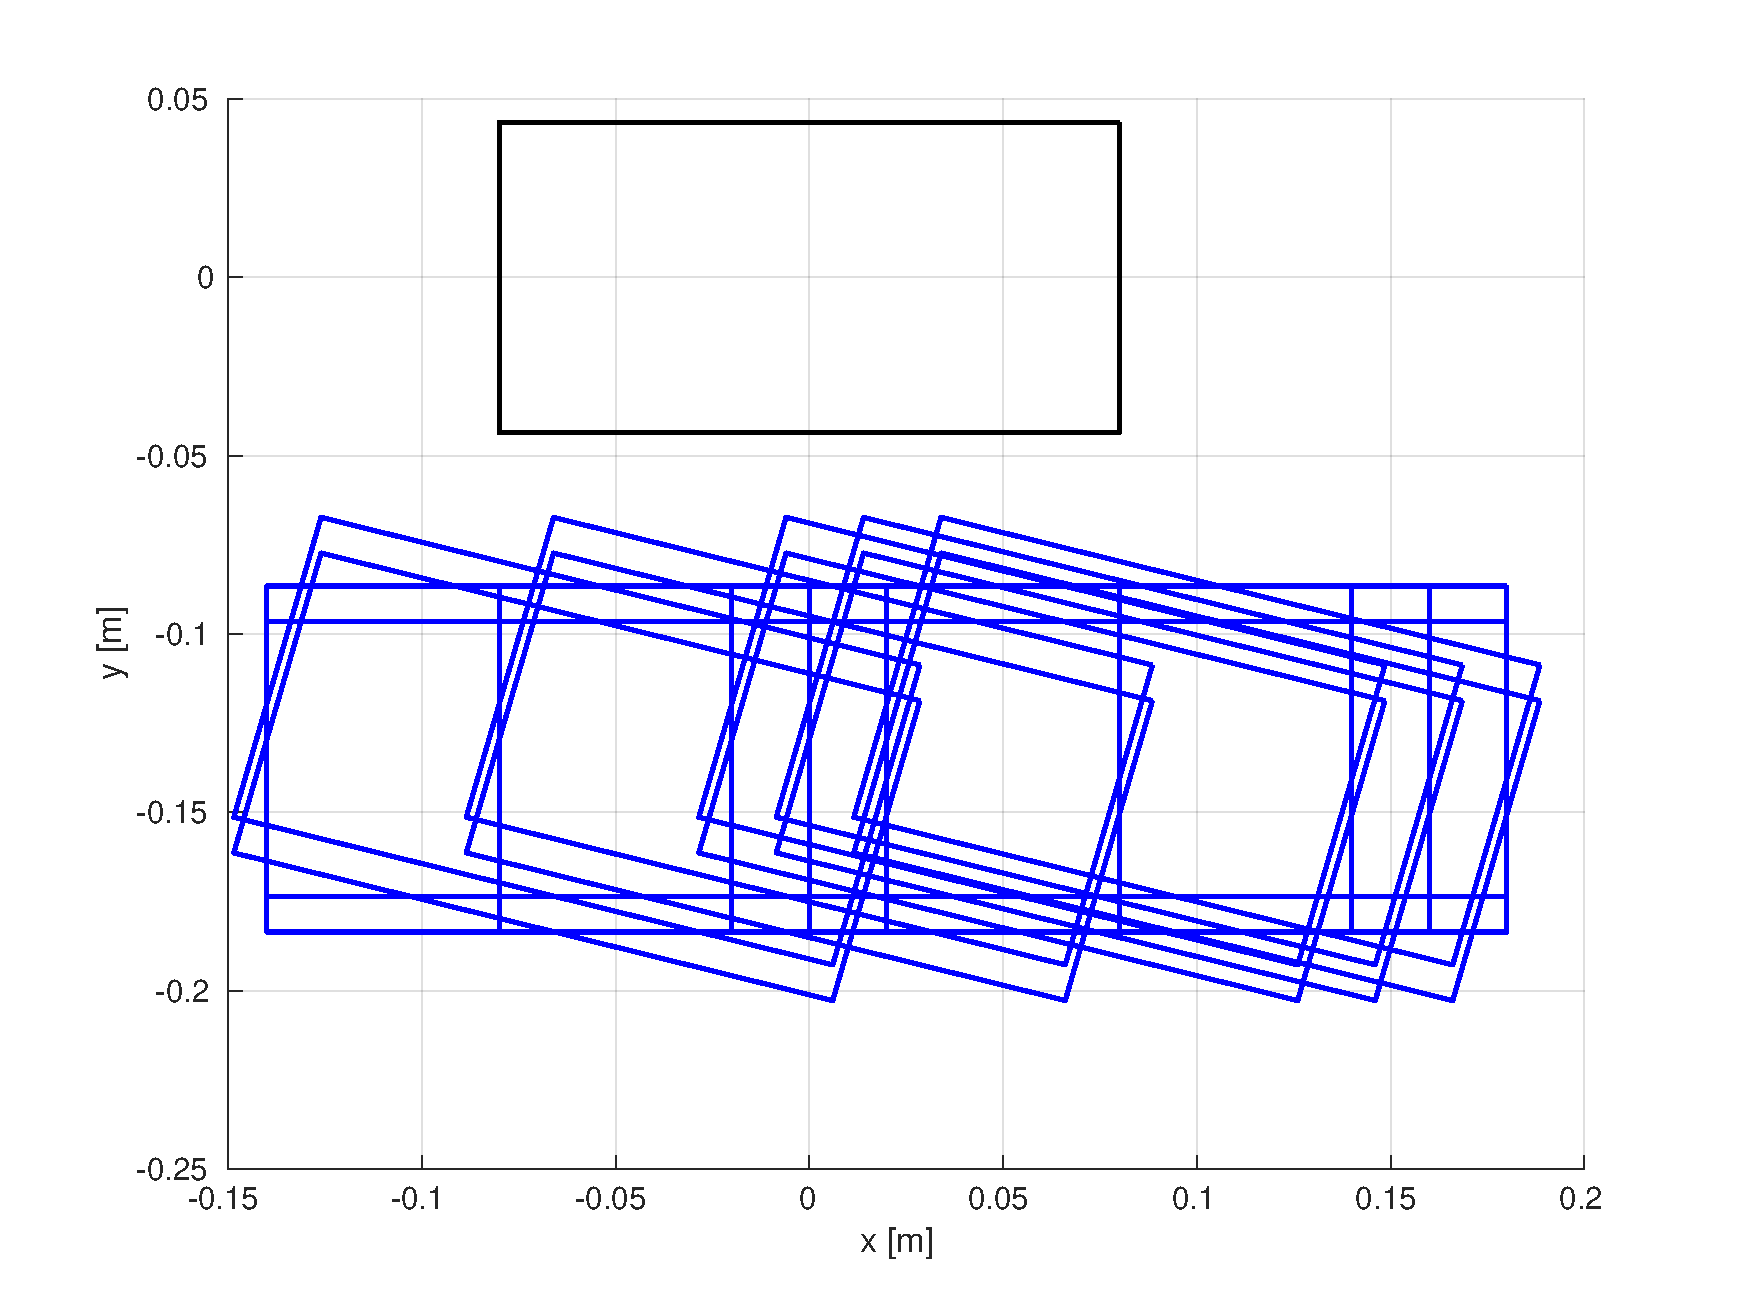
\includegraphics[width=\textwidth]{figures/catalogue-primitives.pdf}
    \caption{The catalogue of primitives (blue color) specifies the possible
        poses of the
        candidate footstep $\bff^{\rm cand}$ with respect to the pose of the 
        current support foot $\bff_{\rm sup}^{\rm near}$. The figure shows the 
        case where the left foot is the support foot. The catalogue for the 
        case where the right foot is the support foot is specular. The $z$
        coordinate of a candidate footstep can be retrieved directly from 
        the elevation map $\mathcal{M}_z$.}
    \label{fig:catalogue-primitives}
\end{figure}
The footstep planning hyperparameters have been set in the following way:
the goal region has been defined as a circle of radius $0.01 {\rm m}$,
$\alpha=1$,
$\Delta z_{max}=0.045 {\rm m}$, $h_{\min}=0.02 {\rm m}$,
$h_{\max}=0.07 {\rm m}$, $\Delta h=0.01 {\rm m}$.
The resolution of $\mathcal{M}_z$ has been set to $0.01 {\rm m}$ when using maps 
generated by \texttt{elevation\_mapping} and to $0.02 {\rm m}$ when using maps 
generated manually.

